% TOdO: Outline that binary output is recommended by the client. It is possible to have more complicated output for Other models.
% Here we present our results from trying to use the following models to extrapolate a time series.
% Classification models output in binary categories: increase or decrease in value, and are therefore less precise.
Here we describe four simpler machine learning models we used for comparison with LLM results: Linear Regression, Multilayer Perceptron, Convolutional Neural Network, Residual Neural Network. The descriptions include a short, technical overview of how the models work. In \autoref{chap:results} we present the results of time series extrapolation using those models.

In the below descriptions, \textbf{overfitting} refers to a phenomenon when a model learns from the training data too closely or exactly, thereby making it less generalizable to new data. See  figure  \autoref{fig:overfitting} for an illustration of the phenomenon. Both the figure and the description are taken from Wikipedia \cite{overfitting}.
\begin{figure}[h!]
	\centering
	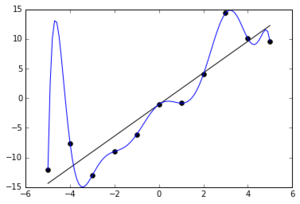
\includegraphics[width=0.5\linewidth]{"pictures/overfitted_data.png"}
	\caption{\textit{Noisy (roughly linear) data is fitted to a linear function and a polynomial function. Although the polynomial function is a perfect fit, the linear function can be expected to generalize better: if the two functions were used to extrapolate beyond the fitted data, the linear function should make better predictions.}}
	\label{fig:overfitting}
\end{figure}
% \section{How we describe models}
% Below, in the chapter "Other models" we describe several models we tried to use for the task of predicting prices. The descriptions include the following:
% \begin{itemize}
% 	% \item \textbf{Relevant literature:} 
% 	\item \textbf{Description:} a short description of how the model works and how it is trained.
% 	\item \textbf{Motivation:} what the model is usually used for and why we chose to try it out.
% 	\item \textbf{Features and limitations:} some advantages and benefits of the model, as well as its disadvantages and drawbacks.
% 	\item \textbf{Parameters:} the description of the parameters of the model and how they affect its training.
% 	\item \textbf{Metrics:} how we measured the results of the training and testing of the model.
% 	\item \textbf{Data used:} what combinations of parameters of the model we tested and on what datasets we trained and tested the model.
% 	\item \textbf{Preprocessing:} how the datasets used were preprocessed for training and testing of the model.
% 	\item \textbf{Analysis:} an analysis of our results of our training and testing of the model compared with the results obtained in literature.
% 	\item \textbf{Picture:} a picture or a plot demonstrating the results obtained from testing the model.
% \end{itemize}











% \section{Random forest}
% A random forest \cite{random_forest} is a machine learning model for classification and regression tasks introduced by Leo Breiman in 2001. A random forest is an ensemble of individual tree predictors, each of which depends on a random vector, chosen independently and with the same distribution for every tree. The results from individual trees are then aggregated into the overall result of the model - for classification tasks it is the mode of individual classifications and for prediction tasks it is the mean average of individual predictions.

% The error of forest prediction converges as such as the quantity of trees in the forest increases. The error of forest prediction depends negatively on the accuracy of individual trees and positively on the correlation between them.

% An individual tree is constructed in the following way: a \textbf{sample} - random subset of the dataset - is selected. This and only this subset is used in growing the tree.
% Then, for each node, a random subset of features is chosen. A best split is chosen using the \verb|criterion| function, based on the chosen features of the sample. Then each tree is grown to maximum depth (until all leaves have one datapoint, for classifier trees).

% Below is the list of parameters that influence the growth of trees:

% \begin{itemize}

% 	\item The \verb|num_lags| parameter is the number of previous datapoints taken into account for individual predictions - if \(k=\) \verb|num_lags|, then datapoints \([n-k, n)\) are used to predict price at \(n\). The larger the \verb|num_lags| the more of past data the model takes into account.

% 	\item The \verb|n_estimators| parameter (number of estimators) describes the number of trees grown in the forest. Increasing the number of trees increases the accuracy of the model, but it also increases the computational cost.

% 	\item The \verb|max_features| parameter (number of features) specifies the the number of features of the data considered for a split at each node while growing an individual tree. A higher value of \verb|max_features| may capture more information about the data at the risk of growing more correlated trees, thereby decreasing its randomness and ability to adapt to new data, causing overfitting.

% 	\item The \verb|criterion| parameter describes the function used by the model to calculate a quality of a split at a given node

% \end{itemize}


% The generalization error for forests converges a.s. to a limit
% as the number of trees in the forest becomes large.
% The generalization error of a forest of tree classifiers
% depends on the strength of the individual trees in the
% forest and the correlation between them. Using a
% random selection of features to split each node yields
% error rates that compare favorably to Adaboost
% (Freund and Schapire[1996]), but are more robust with respect to noise. Internal estimates monitor error, strength, and correlation and these are used to show the response to increasing the number of features used in the splitting. Internal estimates are also used to measure variable importance. These ideas are also applicable to regression.

% \subsection{Results}
% TBA
% % TODO reference to the data sets chapter
% The model was trained and tested on the simple property sales dataset.
% The model was trained to classify whether the next price will be higher or lower than the previous one, based on the sequence of prices spanning the last \verb|num_lags| days.
% The combinations of following parameters were tried

% \noindent
% \begin{itemize}
% 	\item \verb|num_lags|: [1, 5, 10, 13, 25, 40, 50]
% 	\item \verb|n_estimators|: [20, 50, 100]
% 	\item \verb|max_features|: [2, 4, 8]
% 	\item \verb|criterion|: ["gini", "entropy", "log\_loss"]
% \end{itemize}

% % TODO Are all parameters independent? Explain better how this behaves.
% The accuracy of the models ranged from 0.749 to 0.827. The main influence seems to be the lag number - the optimal being around 10. Then slightly better were those models with \verb|max_features| equal to 4, and number of trees greater or equal to 50. The criterion didn't seem to play a significant role. See figure \ref{fig:random_forest_fig} below.

% \begin{figure}[h!]
% 	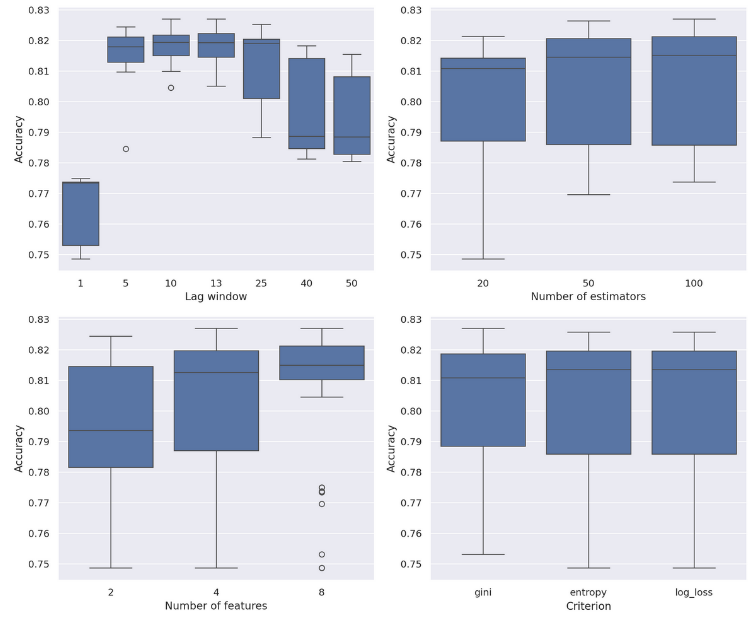
\includegraphics[width=\linewidth]{"pictures/random_forest_results.png"}
% 	\caption{Results of random forest experiment.}
% 	\label{fig:random_forest_fig}
% \end{figure}















\section{Linear regression}

% Logistic regression \cite{logistic_regression} is a statistical method used for binary classification problems, where the outcome variable has one of two possible values. It models the probability that a given input point belongs to a certain class.

% In the below description, \(n\) denotes the size of the training dataset. For our case of predicting time series, an input vector \(x_i\) is a subseries of datapoints of length \verb|num_lags|, for which the output \(y_i\) is a prediction whether the datapoint following \(x_i\) will have a higher or lower price than the previous datapoint. Therefore, in the below description, \(d = \verb|num_lags|*k\), where \(k\) is the number of features of an individual datapoint.

% With that in mind, the general formulation of the logistic regression model is as follows:

% Given a set of \(n\) observations \(\{(x_i, y_i)\}_{i=1}^n\), where \(x_i \in \mathbb{R}^d\) represents the feature vector and \(y_i \in \{0, 1\}\) represents the binary outcome, the logistic regression model predicts the probability of the outcome being 1 (positive class) as:

% \[
% 	P(y = 1 \mid x) = \frac{1}{1 + e^{-(\beta_0 + \beta_1 x_1 + \beta_2 x_2 + \cdots + \beta_d x_d)}}
% \]

% where \(\beta_0\) is the shift term,
% %intercept term (i.e. representing the shift of the baseline probability)
% and \(\beta_1, \beta_2, \ldots, \beta_d\) are the coefficients corresponding to the \(d\) features.

% The model is trained by maximizing the likelihood function, which measures the probability of observing the given data as a function of \(\beta\) parameters. The likelihood function for logistic regression is given by:

% \[
% 	L(\beta) = \prod_{i=1}^n P(y_i = 1 \mid x_i)^{y_i} (1 - P(y_i = 1 \mid x_i))^{1 - y_i}
% \]

% To simplify computation, the log-likelihood function is often used:

% \[
% 	\ell(\beta) = \log(L(\beta)) = \sum_{i=1}^n \left[ y_i \log(P(y_i = 1 \mid x_i)) + (1 - y_i) \log(1 - P(y_i = 1 \mid x_i)) \right]
% \]

% The optimal parameters \(\beta\) are estimated by maximizing the log-likelihood function using numerical optimization techniques such as gradient descent.

\emph{Linear regression} \cite{linear_regression} is a statistical method used for predicting the value of a continuous outcome variable based on one or more input features. It models the relationship between the input features and the continuous outcome by fitting a linear function to observed data.

In the context of predicting time series, an input vector \(x_i\) is a subseries of data points of length \textit{seq\_len}, for which the output \(y_i\) is a prediction of the actual value of the data point following \(x_i\). Therefore, in the description below, the number of features of an input vector is \(d = \textit{seq\_len}\).

With that in mind, the general formulation of the linear regression model is as follows:

Given a set of \(n\) observations \(\{(x_i, y_i)\}_{i=1}^n\), where \(x_i \in \mathbb{R}^d\) represents the feature vector and \(y_i \in \mathbb{R}\) represents the continuous outcome, the linear regression model predicts the value of \(y\) as
\[
	\hat{y} = \beta_0 + \beta_1 x_{i,1} + \beta_2 x_{i,2} + \cdots + \beta_d x_{i,d},
\]
where \(\beta_0\) is the intercept term, and \(\beta_1, \beta_2, \ldots, \beta_d\) are the coefficients corresponding to the \(d\) features.

The model is trained to minimize the residual sum of squares (RSS), which measures the discrepancy between the observed values \(y_i\) and the predicted values \(\hat{y}_i\). The RSS is given by
\[
	RSS(\beta) = \sum_{i=1}^n (y_i - \hat{y}_i)^2 = \sum_{i=1}^n \left(y_i - (\beta_0 + \beta_1 x_{i,1} + \beta_2 x_{i,2} + \cdots + \beta_d x_{i,d})\right)^2,
\]
where \(n\) denotes the number of predicted values.

To find the optimal parameters \(\beta\), the RSS is minimized using analytical methods such as the normal equation or numerical optimization techniques such as gradient descent.





% % TODO: redo the description and results

% Logistic regression \cite{logistic_regression} is a statistical model used for binary classification.
% It calculates the probability of whether a datapoint classifies to one class.
% During training of the model a sigmoid function of features of data is calculated that best fits the provided training dataset.

% %TODO: is n = num_lags? what is n
% More precisely, the model calculates the function \(Y(X) = \frac{1}{1+e^{-z}}\), where
% \begin{itemize}
% 	\item \(z = B_0 + B_1\cdot X_1 + \ldots + B_n\cdot X_n\),
% 	\item \(X_1, \ldots, X_n\) are features of data \(X\),
% 	\item \(B_0, B_1, \ldots, B_n\) are parameters of the model.
% \end{itemize}
% Function \(Y\) assumes values only in the range \((0,1)\).
% If \(Y(X) >= 0.5\), the model classifies the datapoint as 1 (in our model below - the price will be higher). If the converse is true, the datapoint is classified as 0 (the price will be lower).

% % TODO: what is the Maximum Likelihood Function?
% During training the parameters \(B_0, B_1, \ldots, B_n\) are chosen using Maximum Likelihood Estimation function, so that the results of the \(Y\) function best fit the training dataset.

% \subsection{Results}
% TBA


% Two models have been trained.
% The first one is trained to predict if the next price in the dataset wil be higher than the previous one, provided with a sequence of prices spanning over the last \verb|num_lags| days.
% The second one does the same but operates on monthly averages instead of single records (for this, the dataset was averaged over subsuquent months).
% % TODO: Which data set? Why is 40 optimal?
% The first model proved to be more precise with an accuracy of 82\% for an optimal value of k of around 40 (Fig \ref{fig:logv1}). At the same time the second model only scored 75\% (Fig \ref{fig:logv2}).

% % TODO: Why do you wants to predict next price? There was nothing about that in random forest
% However, simply predicting whether the price will be higher or lower is much easier then predicting the actual next price.
% % TODO: IT is not poor if comppared to random forest. Maybe you you should explain why the random forest does perform poorly.
% Additionally, logistic regression assumes an independence of datapoints from each other, wherefore it performs poorly for time series datasets.
% Therefore this model is insufficient for our purpose.

% \begin{figure}[h!]
% 	\centering
% 	\begin{subfigure}[b]{0.4\linewidth}
% 		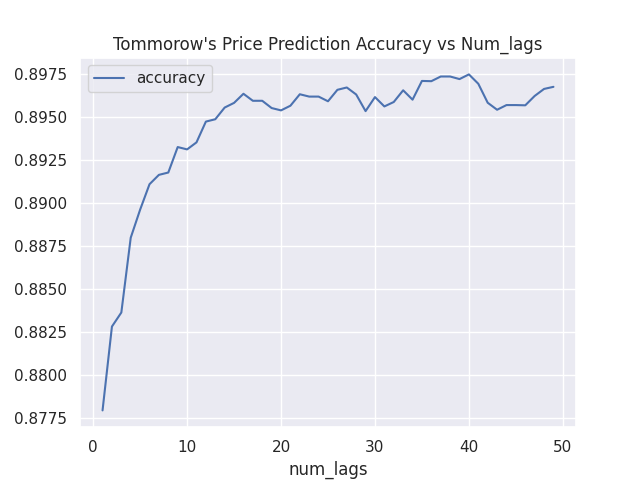
\includegraphics[width=\linewidth]{pictures/logistic-regression-v1.png}
% 		\caption{Day-by-day prediction.}
% 		\label{fig:logv1}
% 	\end{subfigure}
% 	\begin{subfigure}[b]{0.4\linewidth}
% 		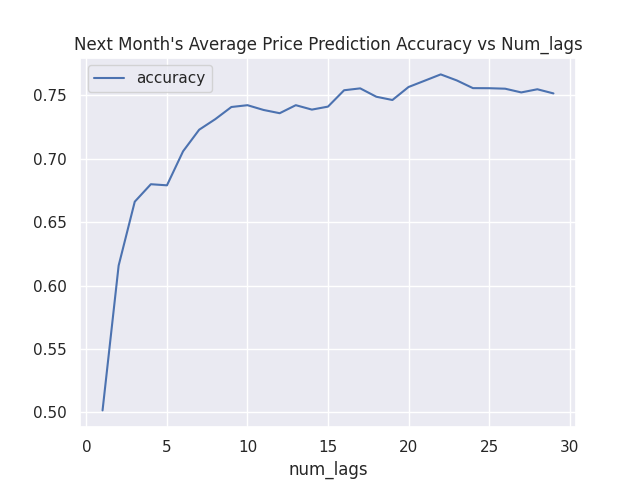
\includegraphics[width=\linewidth]{pictures/logistic-regression-v2.png}
% 		\caption{Month-by-month prediction.}
% 		\label{fig:logv2}
% 	\end{subfigure}
% 	\caption{Plots of two models of logistic regression.}
% 	\label{fig:logistic-regression}
% \end{figure}












% \section{Support vector machine}

% % TODO: make a diagram

% Support Vector Machines (SVMs) are supervised learning models used for classification and regression tasks. They are particularly well-suited for binary classification problems. The main idea behind SVMs is to find the optimal hyperplane that maximally separates the data points of different classes in the feature space.

% A hyperplane is defined by the equation
% \[
% 	\mathbf{w} \cdot \mathbf{x} + b = 0,
% \]
% where \( \mathbf{w} \) is the weight vector and \( b \) is the bias term. The optimal hyperplane is the one that maximizes the margin, which is the distance between the hyperplane and the nearest datapoints from either class, known as support vectors.

% To find this optimal hyperplane, SVM solves the following optimization problem:
% \[
% 	\min_{\mathbf{w}, b} \frac{1}{2} \|\mathbf{w}\|^2
% \]
% subject to the constraint:
% \[
% 	y_i (\mathbf{w} \cdot \mathbf{x}_i + b) \geq 1, \quad \forall i
% \]
% where \( y_i \in \{-1, 1\}\) is the class label of the \( i \)-th data point \( \mathbf{x}_i \).

% For non-linearly separable data, SVM can employ kernel functions to map the input features into a higher-dimensional space where a linear separation is possible.
% %Commonly used kernel functions include the linear, polynomial, and radial basis function (RBF) kernels.
% % Support vector machine \cite{support_vector_machine} is a model for machine learning classification problems, due to their high generalization abilities and applicability to high-dimensional data.

% % The model construes datapoints as high-dimensional vectors and finds the best hyperplane that divides the two classes the data is classified into. The goal of training is to find the hyperplane with the greatest margin - that is, the greatest distance from the closest vectors, called the support vectors.

% \subsection{Parameters}
% \begin{itemize}
% 	\item \textbf{Kernel:}\footnote{Note that the word 'kernel' here is \textbf{not} meant in the linear algebra sense of part of the domain that is transformed to zero.} The model uses a kernel function to transform the space of data points which are not separable by a hyperplane, into one where they are separable.

% 	      The following description is from \cite{support_vector_machine} from page 4. \( X \) and \(Z\) are, respectively, the original input space and the transformed, high-dimensional space.


% 	      Roughly speaking, a kernel \( K(x, y) \) is a real-valued
% 	      function \( K : X \times X \rightarrow \mathbb{R} \) for which there exists a
% 	      function \( \Phi : X \rightarrow Z \), where \( Z \) is a real vector space,
% 	      with the property \( K(x, y) = \Phi(x)^T \Phi(y) \). The
% 	      kernel \( K(x, y) \) acts as a dot product in the space \( Z \).
% 	      %In the SVM literature \( X \) and \( Z \) are called, respectively, input space and feature space. %\cite{support_vector_machine} 

% 	\item \textbf{C value:} The \(C\) value specifies how accurate the model should be, that is how much it should avoid misclassifications, versus how wide the margins should be. A lower value of \(C\) corresponds to wider margins, but potentially more misclassifications. % TODO: in what metric: %, count?

% 	      % TODO: Better describe the gamma
% 	\item \textbf{Gamma:}
% 	      %The gamma parameter is used by the non-linear kernel functions to specify how quickly the kernel specifies how much influence individual training datapoints should have. The \verb|scale| value of gamma means that gamma is scaled automatically to fit the size of the dataset.
% 	      The \( \gamma \) parameter is a component of non-linear kernel functions, (e.g. the Radial Basis Function (RBF) kernel: \(K(\mathbf{x}_i, \mathbf{x}_j) = \exp(-\gamma \|\mathbf{x}_i - \mathbf{x}_j\|^2)\). It determines how
% 	      %far the influence of a single training example reaches, effectively controlling the shape and smoothness of the decision boundary. 
% 	      influential a single datapoint has in shaping the optimal boundary
% 	      A high \( \gamma \) value causes the influence of each training point to be very localized, resulting in a more complex and tailored model that can capture intricate patterns in the data, but with a higher risk of overfitting. A low \( \gamma \) value means that the influence of each training point extends further, producing a smoother and simpler decision boundary that may generalize better to unseen data but be less accurate.
% \end{itemize}
% A model was trained to predict whether the next price will be higher or lower than the previous one.

% What was used is Support Vector Regression, which is a modification of the idea of Support Vector Machine for the purposes of regression tasks, where instead of finding a hyperplane, 

% \subsection{Results}
% TBA

% The model was tested using two metrics: Mean Squared Error and R-squared.

% For the support vector machine there were overall nine models tried:

% \begin{itemize}
% 	\item three kernels: \verb|rbf|, \verb|poly|, \verb|sigmoid|
% 	\item one gamma: \verb|scale|
% 	\item three C values: 0.1, 1.0, 10.0
% \end{itemize}
% % TODO Be precise. What does it mean much better.
% The `poly` kernel worked much better than both `rbf` and `sigmoid`, which both worked equally badly.
% % TODO Be precise. Compared to what. What are the expectations?
% Overall, though, the statistics for every model were terrible. The value of `C` has had very little impact and only on `rbf` kernel.

% Support Vector Machine model doesn't perform well in this task, as can be seen in the results (Fig \ref{fig:svm}). Overall, Support Vector Machins don't perform well with large datasets, which will be part of our endeavour.

% % TODO It is not clear, what is presented on this picture.
% \begin{figure}[h!]
% 	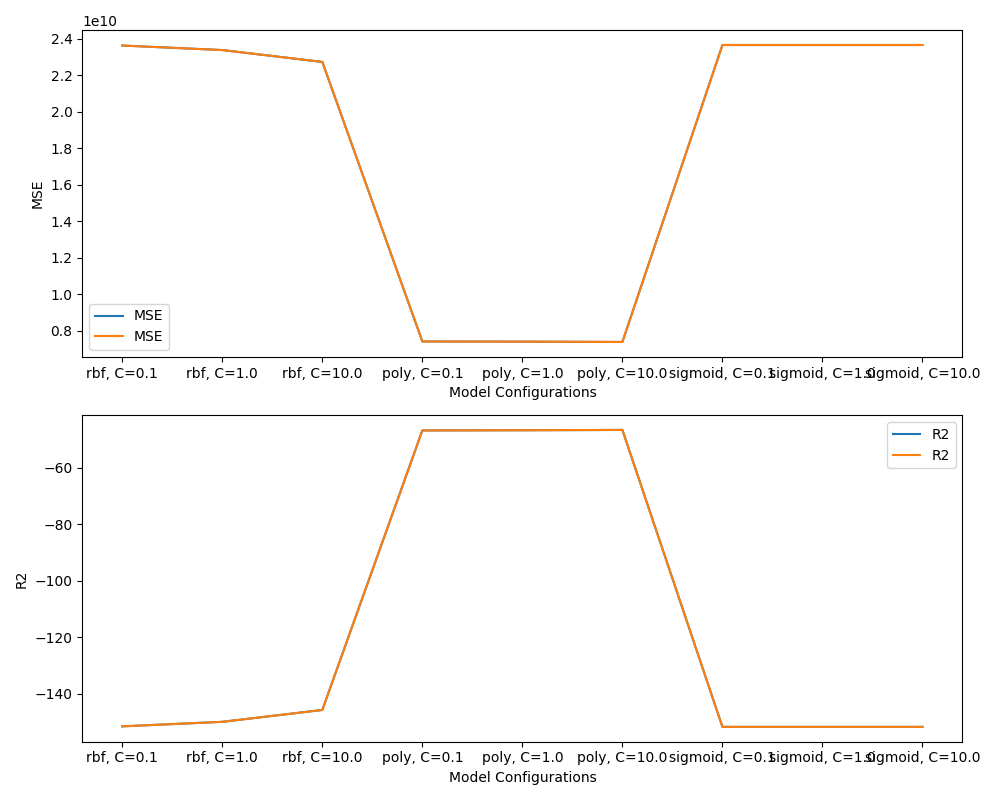
\includegraphics[width=\linewidth]{"pictures/svm_models_results.png"}
% 	\caption{Results of support vector machine experiment.}
% 	\label{fig:svm}

% \end{figure}



















\section{Multilayer Perceptron}
The \emph{Multilayer Perceptron} (MLP) \cite{multilayer_perceptron} is a \emph{feedforward neural network}, that is made up of multiple layers of nodes in a directed graph, where each node from one layer is connected to all the nodes from the previous one.
MLPs are widely used in pattern recognition, classification, and regression problems due to their ability as networks to model complex nonlinear relationships in the input data.
An MLP consists of an input layer of neurons, one or more hidden layers, and an output layer.
Each node, except for those in the input layer, is a neuron that uses a nonlinear activation function to combine inputs from the previous layer and an additional \emph{bias term}.

\subsection{Structure of an MLP}

An MLP is made up of the following components:
\begin{itemize}
	\item \textbf{Input Layer:} The first layer of the network, which receives the input data to be processed. Each neuron in this layer represents a feature of the input data.
	\item \textbf{Hidden Layers:} One or more layers that perform computations on the inputs received and pass their output to the next layer. The neurons in these layers apply activation functions to their inputs to introduce nonlinearity.
	\item \textbf{Output Layer:} The final layer that produces the output of the network.
\end{itemize}

\subsection{Forward Propagation}

The process of computing the output of an MLP is called forward propagation.
In this process, the input data is passed through each layer of the network, transforming the data as it moves through. The output of each neuron is computed as follows:
\begin{equation}
	a^{(l)}_j = \phi\left(\sum_{i} w^{(l)}_{j,i} a^{(l-1)}_i + b^{(l)}_j\right),
\end{equation}
where
\begin{itemize}
	\item $a^{(l)}_j$ is the activation of the $j$-th neuron in the $l$-th layer;
	\item $\phi$ denotes the activation function, e.g. ReLU (\autoref{relu}), Softmax;
	\item $w^{(l)}_{j,i}$ represents the weight from the $i$-th neuron in the $(l-1)$-th layer to the $j$-th neuron in the $l$-th layer;
	\item $b^{(l)}_j$ is the bias term for the $j$-th neuron in the $l$-th layer;
	\item $a^{(l-1)}_i$ is the activation of the $i$-th neuron in the $(l-1)$-th layer.
\end{itemize}

\subsection{Backpropagation and Training}

To train an MLP, the backpropagation algorithm is used.
This algorithm adjusts the weights and biases of the network to minimize the difference between the actual output and the expected output.
The process involves computing the gradient of a \emph{loss function} with respect to each weight and bias in the network, and then using these gradients to update the weights and biases in the direction that minimizes the loss.
The loss function measures the error between the predicted output and the actual output. In our experiments, we used MSE as a loss function. The update rule for the weights is given by
\begin{equation}
	w^{(l)}_{j,i} \leftarrow w^{(l)}_{j,i} - \eta \frac{\partial \mathcal{L}}{\partial w^{(l)}_{j,i}},
\end{equation}
where
\begin{itemize}
	\item $\eta$ is the learning rate. If it is too small, the model will train very slowly and may get stuck in local minima. If it is too large, it might not converge.
	\item $\frac{\partial \mathcal{L}}{\partial w^{(l)}_{j,i}}$ is the partial derivative of the loss function $\mathcal{L}$ with respect to the weight $w^{(l)}_{j,i}$.
\end{itemize}
Similar updates are made for the biases.

Through iterative training involving forward propagation, loss calculation, and backpropagation, the MLP learns to approximate the function that maps data inputs to desired predictions.

% \subsection{Results}
% TBA
% % TODO This does not make sense if you test different models on different data sets.
% The model has been trained and tested on the google dataset.
% The results can be seen below (Fig \ref{fig:mlp}).
% % Model Architecture id is given by:


% \begin{figure}[h!]
% 	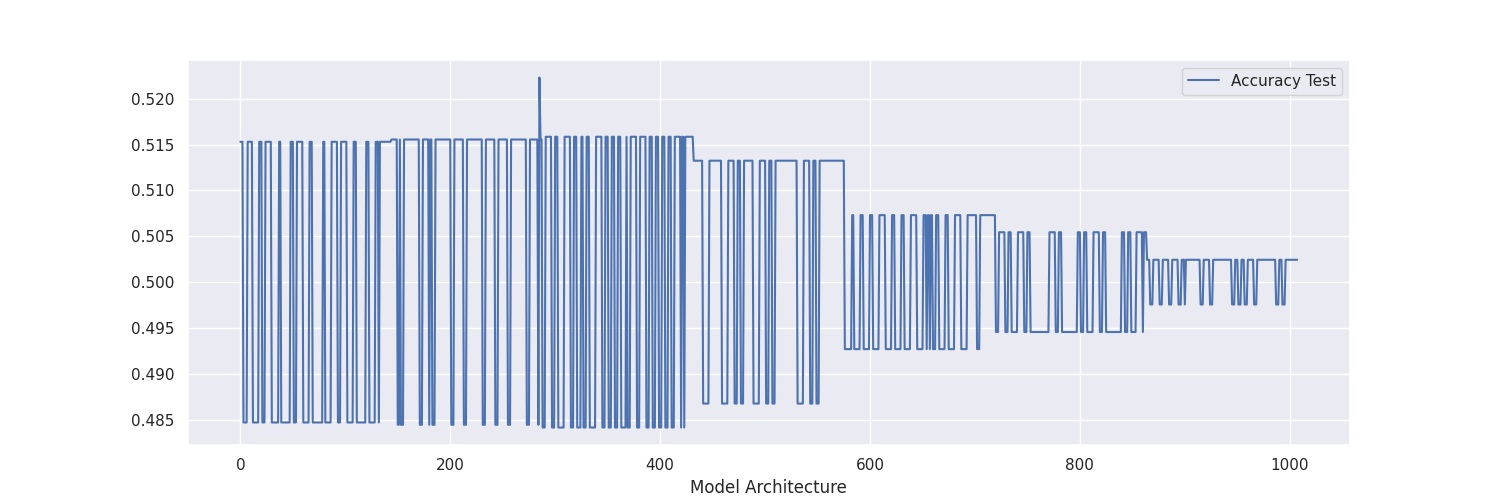
\includegraphics[width=\linewidth]{"pictures/mlp_res.png"}
% 	\caption{Results of multilayer perceptron experiment.}
% 	\label{fig:mlp}

% \end{figure}


























\section{Convolutional neural network}
Convolutional Neural Networks (CNNs) \cite{convolutional_neural_network} are a class of deep neural networks, highly effective for analyzing visual imagery. They employ a mathematical operation called convolution, which allows them to efficiently process data in a grid-like topology, such as images.
%In the CNN the input is construed as consisting of several \emph{channels}, i.e. aspects of the input data (e.g. RGB for images).

\subsection{Architecture of Convolutional Neural Networks}
A typical CNN architecture comprises several layers that transform the input image to produce an output that represents the presence of specific features or class labels. The layers found in a CNN are:

\subsubsection{Convolutional Layer}
The convolutional layer applies a set of learnable filters to the input. Each filter activates specific features at certain spatial positions in the input. Mathematically, the convolution operation of each filter is defined as follows:
\[f(x, y) = (g * h)(x, y) = \sum_m\sum_n g(m,n) \cdot h(x-m, y-n),\]
where \(f(x, y)\) is the output, \(g\) is the filter, \(h\) is the input image, and \(*\) denotes the convolution operation. \(x\) and \(y\) range over output image dimensions; \(m\) and \(n\) range over the filter dimensions.

Following convolution, an \textbf{activation function} is applied to introduce nonlinearity into the model. The Rectified Linear Unit (ReLU) \label{relu} is commonly used:
\[\phi(x) = \max(0, x).\]

For time series forecasting, we use 1-dimensional convolutional neural network, which means that filter has \(1\) row.


\subsubsection{Pooling Layer}
The pooling layer reduces the spatial dimensions (width and height) of the input volume for the next convolutional layer.
%It operates independently on every depth slice of the input and resizes it spatially. 
% A common operation for pooling is max pooling:
% % TODO: what is the range of x y?
% where \(D\) is the set of coordinates in the input, and \(g\) is the input image.

\subsubsection{Fully Connected Layer}
Towards the end of the network, fully connected layers are used, where each input node is connected to each output by a learnable weight.

A simple diagram of the layers can be seen on figure \autoref{fig:cnn-diagram} (from \cite{cnn_diagram_source}). \footnote{In the image: the result of the convolution layer is a stack of output images, one for each filter.}

\begin{figure}[h!]
	\centering
	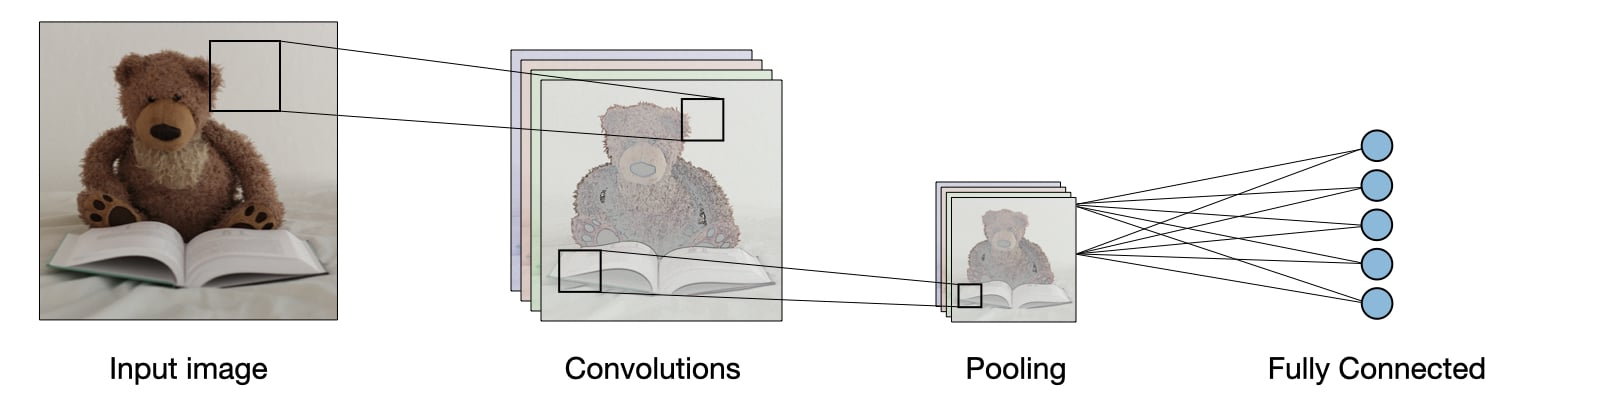
\includegraphics[width=0.5\linewidth]{"pictures/architecture-cnn-en.jpeg"}
	\caption{A simple diagram illustrating the different layers of the network working on an example input image.}
	\label{fig:cnn-diagram}

\end{figure}

% \subsection{Results}
% TBA
% The CNN model has been trained and tested on the simple house sales data.






\section{Residual Neural Network}


A Residual Neural Network (ResNet) is a type of deep learning model specifically designed to mitigate the vanishing gradient problem, where through backpropagation only the last few layers of the network get trained. ResNets introduce skip connections, also known as residual connections, which allow the input of a layer to be directly added to the output of a subsequent layer. This is mathematically expressed as
\[
	\mathbf{y} = \mathcal{F}(\mathbf{x}, \{W_i\}) + \mathbf{x},
\]
where $\mathbf{y}$ is the output of the layer, $\mathcal{F}$ represents the residual mapping to be learned by the layer, $\mathbf{x}$ is the input, and $\{W_i\}$ denote the weights of the layers.

The primary advantage of this architecture is its ability to facilitate the training of deeper networks by preserving the gradient flow through the network during backpropagation. This is achieved by allowing the backpropagation to bypass one or more layers, reducing the risk of gradient vanishing (where update gradients become exponentially small during backpropagation, slowing down training). As a result, ResNets can be trained to greater depths than CNNs, and can have more layers.
% As the number of layers in classic CNN grows, the problem of vanishing or exploding gradient appears.
% It means that gradients become very small (or very large in case of exploding) as they are propagated
% through the layers of the network.

% Residual neural network (ResNet) is a type of CNN that is less subject to this problem.
% It was developed by Kaiming He, Xiangyu Zhang, Shaoqing Ren and Jian Sun in 2015 \cite{residual_neural_network}

% \subsection{ResNet Architecture}


% ResNet uses a technique called skip connections. Skip connection bypasses several layers, so
% that input of one layer is added to the output of some further layer. Blocks of such connections
% are called residual and the network is formed by stacking residual blocks.

% % TODO: explain better, make a diagram.
% The idea is that instead of learning the original mapping of input to output, residual blocks
% learn the difference between output and input, which is called the residual function.

% \subsection{Results}
% TBA

% This model has been trained on GBP/CAD dataset in two versions: not pretrained and pretrained.

% TODO add pictures



















